\chapter{Risultati Sperimentali}
In questo capitolo vengono discussi i risultati degli esperimenti effettuati sul sistema.\\*
Gli esperimenti sono divisi principalmente in due categorie:
\begin{itemize}
	\item Esperimenti \emph{offline}:\\*
	I dati di IMU, Odometro e GPS vengono generati attraverso RTT e passati a un'istanza locale di \texttt{FusionLib}.\\*
	I risultati forniti da SFA vengono mostrati su RTT in forma grafica.\\* Questi esperimenti sono essenzialmente \emph{Integration Test} volti a validare l'implementazione di SFA e vengono eseguiti interamente con RTT, il quale genera un report per ogni esperimento effettuato.\\*
	In figura \ref{fig:rtt} si mostra lo schema logico di un esperimento effettuato con RTT.
	\begin{figure}[h]
		\centering
		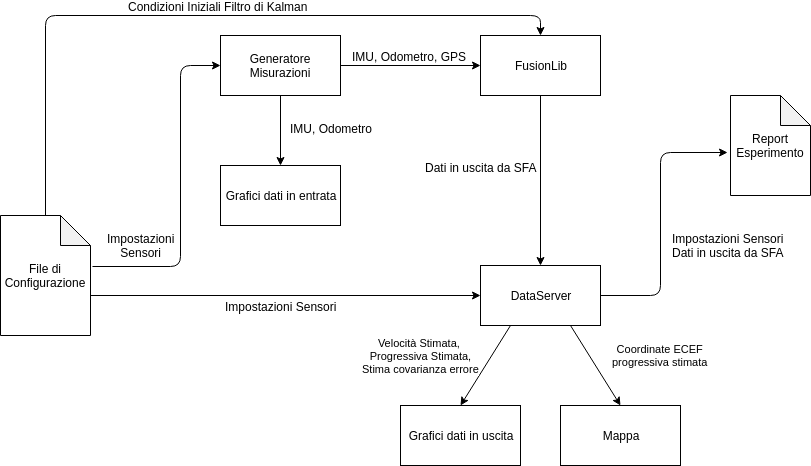
\includegraphics[width=\linewidth]{img/rtt}
		\caption{Esperimenti offline}
		\label{fig:rtt}
	\end{figure}
	\item Esperimenti \emph{online}:\\*
	Il software \texttt{SynthDataGenApp} (SDGA), essenzialmente un'opportuna estrazione di codice da RTT, \`e un software capace di generare i dati di IMU, Odometro e GPS.\\*
	SDGA si comporta come un'astrazione di \texttt{interface-modules}, e le misurazioni prodotte vengono inviate in accordo a \texttt{INPUT\_PROTOCOL} a una scheda \texttt{NVidia TX-Jetson} su cui \`e replicato l'ambiente HW e SW bordo treno. Tali dati sono inviati alla scheda attraverso un'interfaccia \texttt{ethernet}, utilizzata in luogo dell'interfaccia \texttt{loopback} prevista dal sistema reale.\\*La scheda invia i dati in uscita da SFA, attraverso la medesima interfaccia \texttt{ethernet}, al mittente dei dati in entrata in accordo a \texttt{OUTPUT\_PROTOCOL}.\\*In questo caso, l'interfaccia \texttt{ethernet} sostituisce l'utilizzo del modem \texttt{LTE}.\\*
	Questi esperimenti sono essenzialmente \emph{End to End Test} e hanno lo scopo di validare i protocolli di comunicazione.
	\begin{figure}[h]
	\centering
	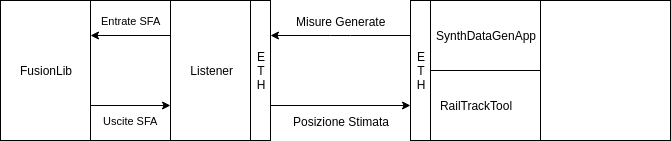
\includegraphics[width=\linewidth]{img/onlinetest}
	\caption{Esperimenti online}
	\label{fig:online}
\end{figure}
\end{itemize}
La linea ferrotramviaria scelta come ambiente di prova \`e la linea \texttt{T1} della Tramvia di Firenze, che collega la stazione di \emph{Villa Costanza}, sita nel comune di Scandicci, all'ospedale di \emph{Careggi}, sito quest'ultimo nel comune di Firenze. La linea \`e mostrata in figura \ref{fig:t1}.\newpage
\begin{figure}[h]
	\centering
	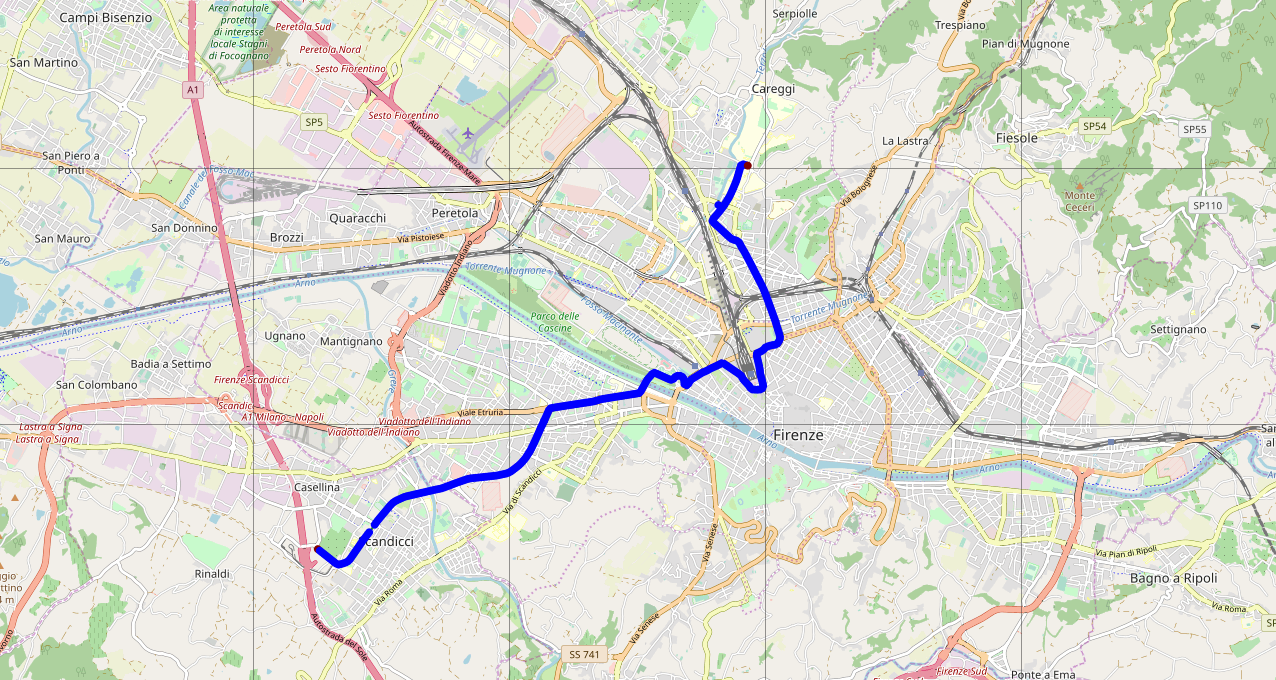
\includegraphics[width=\linewidth]{img/t1}
	\caption{Tramvia di Firenze - Linea \texttt{T1}}
	\label{fig:t1}
\end{figure}

\section{Software impiegati}
In questa sezione vengono descritti i SW utilizzati negli scenari sopra descritti.
\subsection{FusionLib}
Come accennato nel Capitolo 3, \texttt{FusionLib} \`e una \emph{libreria software} che implementa SFA. Tale libreria viene compilata sia su \texttt{Windows 10}, su cui esegue RTT, che su \texttt{Ubuntu 16.04 LTS}, su cui esegue \texttt{listener}. \texttt{FusionLib} \`e pertanto una libreria inclusa da \texttt{listener} e RTT.\\*
Per determinare la posizione del treno lungo la traccia \texttt{FusionLib} utilizza le informazioni ricevute dal chiamante, quindi le misure, combinate con le informazioni della traccia su cui si assume il treno si stia muovendo. Tali informazioni sono salvate in un \emph{database SQL}. Lo schema logico \`e riportato in figura \ref{fig:fulib}.\\*
\begin{figure}[h]
	\centering
	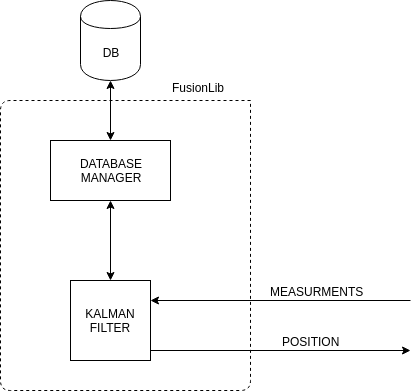
\includegraphics[width=\linewidth]{img/fulib}
	\caption{Architettura logica di \texttt{FusionLib}}
	\label{fig:fulib}
\end{figure}
La traccia entro cui il treno si muove \`e rappresentata da una \emph{spline}. Una \emph{spline} \`e una funzione polinomiale a tratti che interpola una serie di $N$ coppie $(x_i,y_i)$, dette \emph{nodi}, utilizzando differenti funzioni polinomiali per ciascun intervallo $(x_i,x_{i+1})$ per $i = 1,\dots,N-1$.\\*
Nelle figure \ref{fig:spline} e \ref{fig:cos}, si mostra come una spline polinomiale sia in grado di approssimare in maniera accettabile una funzione sufficientemente regolare.\\*
\begin{figure}[h]
	\centering
	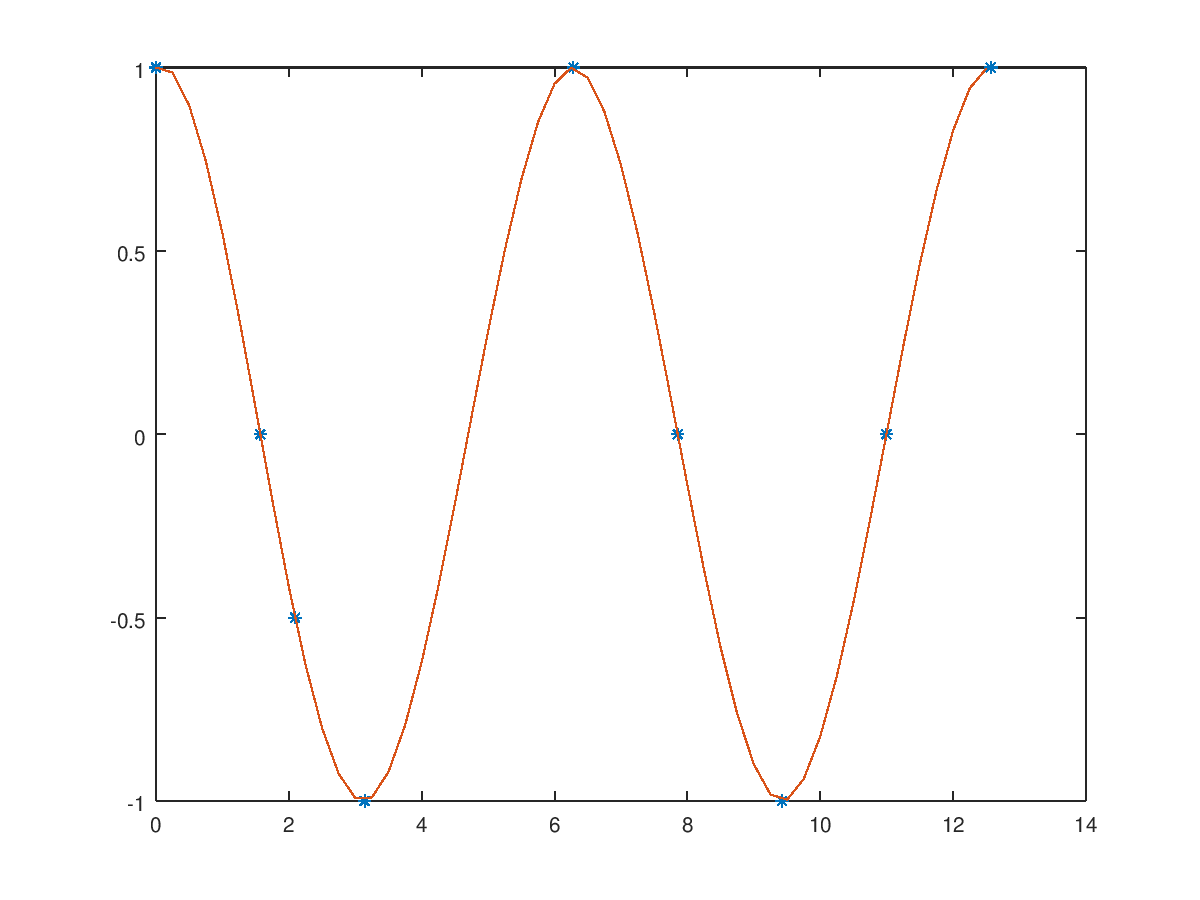
\includegraphics[width=\linewidth]{img/spline}
	\caption{Spline interpolante la funzione $\cos(x)$ nelle ascisse $ \frac{k\pi}{2}\;\; k = 0,\dots,8$}
	\label{fig:spline}
\end{figure}

\begin{figure}[h]
	\centering
	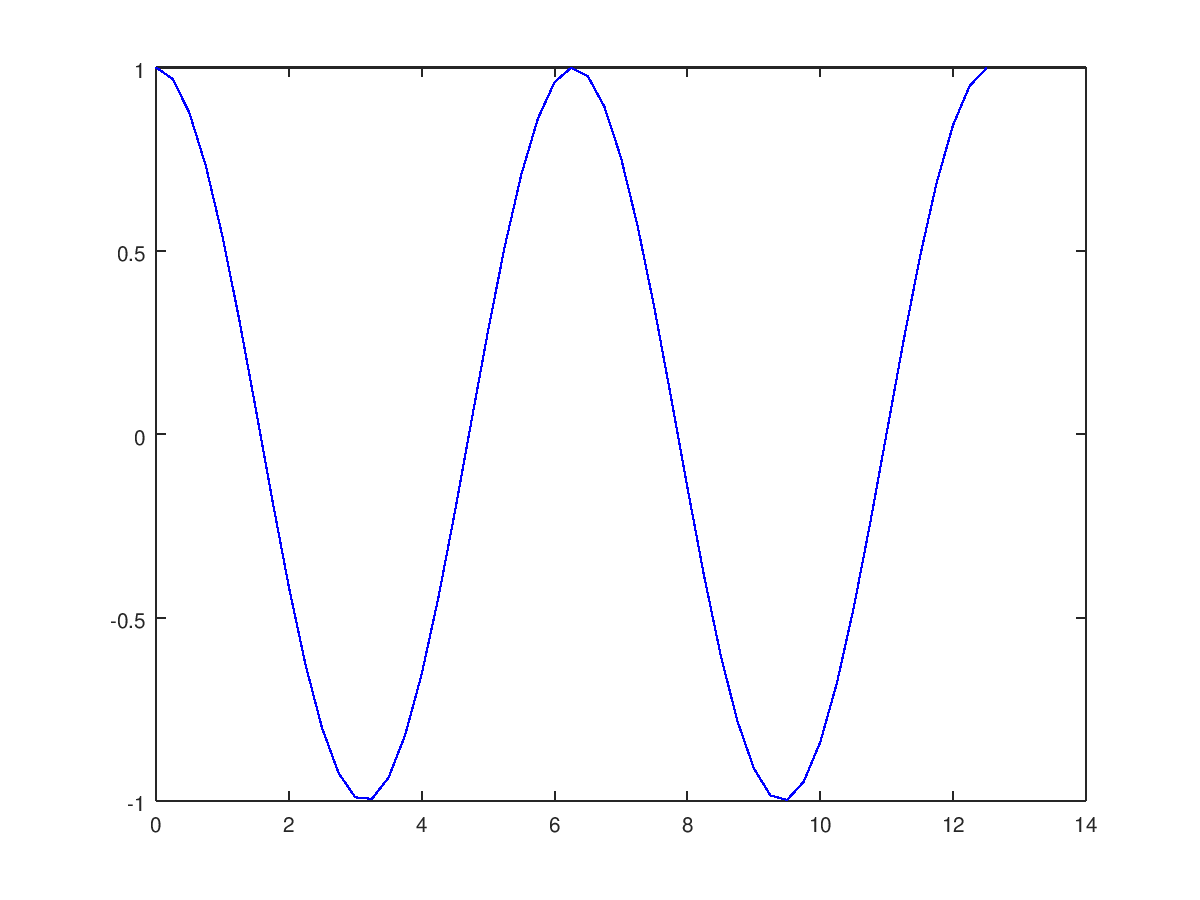
\includegraphics[width=\linewidth]{img/cos}
	\caption{Funzione $\cos(x)$ nell'intervallo reale $[0,4\pi]$}
	\label{fig:cos}
\end{figure}
La logica \`e quella di campionare, per una data traccia, una serie di coppie $(x_i,y_i) = $ \texttt{(longitudine,latitudine)} di punti geografici appartenenti alla traccia. Queste coppie vengono salvate nel database insieme al valore $P_k$ di progressiva chilometrica che caratterizza ciascuna coppia.\\*
Durante l'esecuzione di SFA, il database viene consultato per recuperare il valore corretto delle coordinate geografiche attuali del treno:
\begin{itemize}
	\item La $k-$esima ricezione di misure causa l'aggiornamento del filtro;
	\item L'aggiornamento del filtro produce la $k-$esima stima della progressiva chilometrica attuale: $\hat{x}_k$. La distanza percorsa rispetto all'iterazione precedente \`e data da:
	$$
	D_k = \hat{x}_{k} - \hat{x}_{k-1}
	$$
	\item Dal database vengono recuperate le coppie $(x_0,y_0)$, $(x_1,y_1)$ della traccia, tali per cui:
	\begin{enumerate}
		\item La progressiva chilometrica associata alla coppia $(x_0,y_0)$ \`e il massimo $P_{k}$ tale per cui $P_{k} < \hat{x}_k$
		\item La prorogressiva chilometrica associata alla coppia $(x_1,y_1)$ \`e il minimo $P_{k}$ tale per cui $P_k > \hat{x}_k$
	\end{enumerate}
In altre parole, si \`e determinato l'intervallo della spline in cui il treno \`e stimato trovarsi al passo $k$.\\*
\`E opportuno precisare che 
	le coppie ottenute dal database non sono in formato ECEF, infatti esse sono espresse in gradi. Tuttavia, \`e possibile applicare una nota trasformazione per convertire la coppia $(x_i,y_i) = $ \texttt{(longitudine,latitudine)} nel formato ECEF.
	
	\item Date le coppie individuate, se ne determina il polinomio interpolante\footnote{Si osservi che \`e sempre possibile, a condizione che $x_0 \neq x_1$.}. Sia esso $p(x)$.
	\item Le coordinate \texttt{ECEF} al passo $k$, $(x_k,y_k)$, sono date da:
	$$
	\begin{cases}
	x_k = x_0 + D_k \\
	y_k = p(x_0 + D_k) = p(x_k)
	\end{cases}
	$$
\end{itemize}
\subsection{RTT}
RTT ha pi\`u modalit\`a di funzionamento:
\begin{enumerate}
	\item \texttt{INTERFACE\_EXT\_FILTER}:\\* In questa motalit\`a, RTT funziona come interfaccia verso un'istanza esterna di \texttt{FusionLib} per visualizzare le uscite di SFA su una mappa. I dati sono letti da una \emph{socket} \texttt{UDP} in accordo al protocollo \texttt{OUTPUT\_PROTOCOL}.\\*
	In questo caso RTT ha il ruolo di OBCU.
	\item
	\texttt{INTERFACE\_SENSOR}:\\*
	In questa modalit\`a RTT si interfaccia verso \texttt{interface-modules}, o comunque qualunque processo che sia in grado di fornire misure di IMU, Odometro e GPS via \texttt{UDP}, in accordo al protocollo \texttt{INPUT\_PROTOCOL}. I dati ricevuti vengono inviati alla propria istanza di \texttt{FusionLib} durante un'esecuzione di SFA.\\*
	In questo caso RTT ha il ruolo di \texttt{listener}.
	\item \texttt{STANDALONE}:\\*
	Modalit\`a standard di funzionamento, come descritta in figura \ref{fig:rtt}.\\*
	In questa modalit\`a, RTT genera misure le misure da inviare alla propria istanza di \texttt{FusionLib} per eseguire SFA.\\*
	In questo caso RTT simula l'intero processo del sistema di posizionamento.
\end{enumerate}
La modalit\'a \texttt{INTERFACE\_EXT\_FILTER} viene usata per visualizzare graficamente i risultati degli esperimenti \emph{online}.\\* La modalit\`a \texttt{STANDALONE} viene usata per gli esperimenti \emph{offline}.\\*
Per quanto riguarda la modalit\`a \texttt{INTERFACE\_SENSOR}, essa non ha una particolare applicabilit\`a sperimentale, infatti questa modalit\`a \`e stata principalmente usata per scopi di \emph{debug} dei protocolli di comunicazione. Questo aspetto sar\`a discusso in seguito.
\subsection{Listener}
Modulo in esecuzione su \texttt{NVidia TX-Jetson}, il cui funzionamento \`e stato descritto nel Capitolo 3.\\*
Ricapitolando, \texttt{listener} riceve le misure dei sensori in accordo a \texttt{INPUT\_PROTOCOL} ed esegue SFA, aggiornando il KF con le misure ricevute in ingresso.\\*
Nonappena viene calcolata un'uscita di SFA, questo software \`e incaricato di inoltrare tale uscita a OBCU o a RTT. Negli scenari sperimentali descritti in questo Capitolo, le uscite di SFA verranno inviate a RTT.
\subsection{SDGA}
Semplice software estratto da RTT. Il compito di SDGA \`e generare le misure ed inoltrarle a \texttt{listener}, secondo il protocollo \texttt{INPUT\_PROTOCOL}.
\section{Esperimenti offline}
Lo scopo degli esperimenti offline era quello di validare l'implementazione di SFA e di valutare il suo comportamento al variare dei parametri di configurazione.
\section{Esperimenti online}